


\subsection{参数法（Parametric Approaches）}

\subsubsection{相关数据}


    \begin{itemize}

       
   

        \item \textbf{收益率计算}
        \begin{itemize}
            \item Profit/Loss
            \[ {P/L} = P_t+D_t-P_{t-1} \]


            \item 算术收益率（arithmetic return）
           \[ {r_t} = \frac{{P_t+D_t-P_{t-1}}}{P_{t-1}} =\frac{{P_t+D_t}}{P_{t-1}}-1\]


            \item 几何收益率（geometric return）
            \[ {R_t} = \ln \left( \frac{{P_t+D_t}}{P_{t-1}} \right) = \ln \left( 1+{r_t} \right) \]
            
          
\[
P_t \text{：第 } t \text{ 期资产价格； } D_t \text{：第 } t \text{ 期收到的现金分红（如股息、利息等）。}
\]



            \item \textbf{注意：}
            \begin{itemize}
                \item 当收益率很小时$R_t \approx r_t$，两者之间的差别可以忽略不计；收益率增大时，两者之间的差别会变大。
                \item 算术收益率适用于短期投资；几何收益率考虑了中期收益，适用于长期投资。
                %\item 算术收益率和几何收益率的差异在于时间的影响。
            \end{itemize}
        \end{itemize}
    \end{itemize}

\subsubsection{Value at Risk (VaR) 风险价值}
\begin{itemize}


    \item \textbf{定义}
    \begin{itemize}
        \item 衡量投资组合在一定置信水平下的最大可能损失
        \item 通常以货币单位或收益率表示，存在两个理解角度，如在95\%置信水平下，VaR=1000：
        \begin{itemize}
        \item （1）表示只有5\%的概率损失超过1000。
        \item （2）表示有95\%的概率损失不超过1000。
    \end{itemize}

    \end{itemize}

 
    \item \textbf{特点}
    \begin{itemize}
        \item \textbf{优点}：简单易懂，直观。
        \item \textbf{缺点}：无法反映极端情况，对尾部风险估计不准确。数据的利用效率比较低，代表性不明显。
    \end{itemize}

\item \textbf{ 以参数法(Parametric Approaches)计算VaR。}
        \begin{itemize}
            \item Normal VaR

        \[ VaR=\left| {\mu-z_\alpha \sigma} \right|\]
        \[ VaR=\left| {\mu-z_\alpha \sigma} \right|*P_{t-1}\]
        

\item Lognormal VaR
\[VaR=1-e^{\mu-z_{\alpha} \sigma}\]
\[VaR=(1-e^{\mu-z_{\alpha} \sigma})*P_{t-1}\]


\end{itemize}


\[\mu: \text{均值} \quad \sigma: \text{标准差} \quad Z_{\alpha}: \text{标准正态分布对应置信水平的关键值}
\]

\end{itemize}








\subsubsection{一致性风险度量（Coherent Risk Measures）}

一致性风险度量方法是损失分布的分位数（\(q_p\)）的加权平均。
%即样本对应置信水平的VaR与对应权重的乘积的平均值。
其计算公式为：

   \[M_\Phi = \int_0^1 \Phi(p) q_p \ ， dp\]
\[\Phi(p) \text{ 表示用户指定的权重函数。} \quad q \text{ 表示对应的分位数。} \quad p \text{ 表示置信水平。}\]




\[\text{权重函数公式：}
\Phi_\gamma(p) = \frac{e^{-\frac{(1-p)}{\gamma}}}{\gamma(1 - e^{-\frac{1}{\gamma}})}
\]




\[\gamma\text{是根据客户的风险厌恶程度决定的常数。通常题目会给出，不用计算。}\]



\begin{note}{一级回顾：一致性风险度量的性质}
    \begin{itemize}
        \item 单调性（Monotonicity）：如果一个投资组合的损失大于另一个投资组合的损失，那么它的VaR值也应该大于另一个投资组合的VaR值。
        \item 次可加性（Sub-additivity）：分散投资能降低风险，组合风险不应大于各部分风险之和。
        \item 正齐次性（Positive homogeneity）：风险随持仓线性扩张。如果把资产规模扩大两倍，风险也应扩大两倍。
        \item 平移不变性（Translational invariance）：如果在投资组合中加入一个确定的现金流$\alpha$，你的整体风险应减少$\alpha$。
    \end{itemize}
\end{note}

\subsubsection{Expected shortfall (ES)}
ES（Expected Shortfall），也叫条件 VaR（Conditional VaR），是一致性风险度量方法的特例，表示超过VaR的损失的期望值（平均值）。
\begin{knowledgebox}{CVaR}
    CVaR可以表示很多意思，这里的CVaR是条件VaR（Conditional VaR）的缩写。在信用风险里，
    CVaR是信用VaR（CreditVaR）的缩写；在投资组合里，CVaR是成分VaR
    （Component VaR）的缩写。
    
\end{knowledgebox}

\[
\phi_\gamma{p} =
\begin{cases}
\frac{1}{n} & \text{当损失} > VaR \\
0 & \text{当损失} \leq VaR
\end{cases}
\]

\(\phi_\gamma{p}\)系ES的权重函数，\(n\)是损失大于VaR的样本数，大于VaR 的损失给予相等权重， 而其他数据给予的权重是0。




\subsubsection{理解标准误差的概念}
\begin{itemize}
    \item \textbf{标准误差（standard error）}
    \[SE(q)≈(\frac{p*(1-p)}{n*f(q)^2})^{0.5}\]
      \(p\)是分位数的比例；\(n\)是样本量；\(f(q)\) 是对应的概率密度函数。
      \begin{itemize}
          \item 标准误差越小越好。
          \item 误差会随着样本量的增大而减小。
          \item 分位数越極端，其估計值就越不精確。
      \end{itemize}

      
    


    \item \textbf{置信区间（confidence intervals）}
    
    标准误差可以用于构建置信区间：
      \[
\left[q - z_{\alpha/2} \times SE(q)， q + z_{\alpha/2} \times SE(q)\right]
\]
    
\item \textbf{分位数标准误的特点}
\begin{itemize}
    \item 易于实施，在大样本情况下具有合理性。
\item 依赖于渐进理论且需要大样本量。
\item 可能产生不精确的估计器或宽置信区间。
\item 产生的对称置信区间在极端分位数下具有误导性。
\end{itemize} 



\end{itemize}




 


\subsubsection{分位数——分位数散点图(Quantile-Quantile Plots)}

\begin{itemize}
    

    \item 用参数法计算VaR值，需要满足收益率服从正态分布的前提下。如果使用Normal VaR方法
来计算VaR值，那么算数收益率数据就必须服从正态分布，如果使用Lognormal
VaR方法计算VaR值，那么几何收益率数据就必须服从正态分布。

\item QQ 曲线可以用来分析判断一个分布是否是某一特定的分布。横坐标是特定的理论分布的分位数，比如正态分布的分位数。纵坐标是经验分布的分位数，即未知分布的分位数。


\item QQ曲线为直线表示数据和分布拟合较好，可以确认实际数据来自于这个理
论分布。
\end{itemize}



\begin{itemize}
    \item QQ plots：将经验分布 empirical distribution 的分位数与某个指定分布的分位数进行对比，以确定我们的数据分布是不是我们想要的那个分布。比如，有一组数据，我想看看它是不是正态分布的，这时就可以使用 QQ plots 这种工具。
    \begin{itemize}
        \item 经验分布 empirical distribution：其实就是实际数据形成的分布
        \item 某个指定分布，也称 reference distribution，比如正态分布
    \end{itemize}

    \item QQ plots:
    \begin{itemize}
        \item 横坐标是特定的理论分布的分位数，比如正态分布的分位数。纵坐标是经验分布的分位数。
        
        \item 结论一：QQ plots 近似为线性 linear，表示数据和分布吻合较好
        \begin{itemize}
            \item the empirical distribution matches the reference population【近似直线表示数据和分布吻合较好，也就是真实数据是正态分布的】。如下图
        \end{itemize}
        
        \begin{figure}[H]    % 强制图片在当前位置
            \centering
            
\includegraphics[width=0.5\textwidth]{NQ.png}
            \caption{QQ plots}
            \label{fig:NQ}
        \end{figure}
        
        \item 结论二：QQ plots 呈现非线性 non-linear，尾部出现偏离（肥尾），表示数据和分布吻合不好。
        \begin{itemize}
            \item the empirical distribution does not match the reference population【也就是真实数据不是正态分布的】。如下图
        \end{itemize}
        
        \begin{figure}[H]    % 强制图片在当前位置
            \centering
            
\includegraphics[width=0.5\textwidth]{NQ2.png}
            \caption{QQ plotss}
            \label{fig:NQ2}
        \end{figure}



    \end{itemize}
\end{itemize}



\subsection{非参数方法}

\subsubsection{非参数方法计算VaR}
   

\begin{itemize}

\item 模拟法的假设：


    \begin{itemize}


    \item 基本假设：历史会重演，用历史损失数据得到的VaR值可以在一定程度上代表未来的损失情况。  
    \item  VaR 不满足次可加性。
    \end{itemize}


\item 计算思想： 把损失数据由大到小进行排列， 然后根据置信水平， 确定是第几大损失。

\[
\text{VaR的位置} = n \times \text{显著性水平} + 1
\]


\item 历史模拟法（Historical Simulation）是非参数法计算VaR的典型方法。即把所有损益数据排序，然后查找相应置信水平下对应的损失。要注意查找损失数据的序数问题，这个序数是由（1-α）×n+1决定。α是对应的置信水平，n是数据个数。



%\begin{note}{VaR数据选取}
 %   100个损失数据，损失由大到小排序，95\%的VaR，行业里并无定论采用第五个还是第六个损失数据，当考试同时出现了第五和第六个损失数据的时候，建议以原版书为准，采用第六个损失数据。
%\end{note}

\begin{knowledgebox}{传统历史模拟法}

    

\begin{itemize}
    \item 优点
    \begin{itemize}
    \item 方法简单
    \item 不需要考虑相关系数、协方差和维度诅咒的问题
    \end{itemize}

    \item 缺点
    \begin{itemize}

    \item 数据的离散性不允许估算数据点之间的风险价值率。
    \item 当数据量比较少时，计算结果可能不准确。
    \end{itemize}
\end{itemize}

\end{knowledgebox}




\end{itemize}



\begin{itemize}
    



%\item 但一个明显的缺点是，数据的离散性不允许估算数据点之间的风险价值率。如果有 100 个历史观测值，那么就可以直接估算出 95\% 或 96\% 置信度的风险价值，以此类推。但是，这种方法无法纳入 95.5\% 的置信水平。更一般地说，对于 n 个观测值，历史模拟法只允许 n 个不同的置信水平。

\item 自举法是一种增加样本量的方式，采用有放回的重抽样。

\begin{itemize}
    \item 方法（求ES同理）：
    \begin{itemize}
        \item 第一步，从原始样本中，随机收取一定数据，得出VaR。
        \item 第二步，把上述数据再放入样本。
        \item 第三步，不断重复第一、二步，得到多个VaR。
        \item 最后，对多个VaR，求均值，得到所需的VaR。
    \end{itemize}
    \item 优势：
    \begin{itemize}
        \item 方法非常直观且易于应用
        \item 通常比原始样本估计更准确
    \end{itemize}
\end{itemize}

\item 非参数密度估计法通过线性插值法来估计VaR。它的基本思想是：在每个数据点上放置一个小的核函数（kernel function），然后将所有核函数相加，得到一个平滑的密度函数。常用的核函数有高斯核、均匀核等。
\item 将每个直方图条顶部的中点用直线连接起来的原始数据

\item 其思路是将我们的数据视为来自某种未指定或未知的经验分布函数的样本。这种方法还促使我们面对关于箱宽和箱心位置的潜在重要决策，而这些决策有时会影响我们的结果。除了使用直方图，我们还可以使用朴素估计量或更一般的核函数来表示我们的数据，文献告诉我们核函数是（或应该是）更优的。因此，在整理好我们的“原始”HS数据后，我们需要决定箱宽和中心位置，以及是否使用直方图、朴素估计量还是某种形式的核函数。如果我们在这些问题上做出良好的决策，我们可以希望获得更好的VaR和ES（以及更一般的连贯测量）。

\end{itemize}







\begin{itemize}
    \item 优点
    \begin{itemize}
    \item 直观、简单、便于理解。
    \item 不依赖于严苛的参数假设，不需要考虑相关系数、协方差和维度诅咒的问题
    \item 适应任何类型的仓位
    \item 所用数据常具有可获得性。
    \item 比较灵活，可以加入参数的成分，使之变成半参数法。
    \end{itemize}

    \item 缺点
    \begin{itemize}

    \item 数据的离散性不允许估算数据点之间的风险价值率。
    \item 严重依赖于历史数据
    \item 会产生鬼影效应
    \item 当数据量比较少时，计算结果可能不准确。
    \item ，如果数据周期异常安静，非参数方法通党产生过低的VaR或ES估计，
    反之亦然。
    
    \item 不能很好地捕捉尾部风险。，很难处理极值损失
    \end{itemize}
\end{itemize}

\subsubsection{半参数法或混合法计算VaR}
\begin{itemize}
    \item 根据年龄加权的历史模拟法
    
    \begin{itemize}
            
        \item 根据年龄加权的历史模拟法（Age-Weighted Historical Simulation）， 因为是Boudoukh，Richardson 和Whitelaw这三个人提出的，也叫做BRW法。

\item 这种方法调整的是每一个历史数据的权重（Weighted），不改变损失数据（Loss
Data）。在前面章节，计算 95\%置信水平下的VaR值时，找到的是第六个数。为
什么要找第六个数，而不是找第三个数、第五个数或第十个数呢？是因为我们认
为在这100个数据里，每一个数据都是等权重的，单个数据所占的权重是1\%。所
以前面5个数合起来是5\%。

\item 实际上，100天前的数据，年龄已经较大。年龄较大的数据，不太能代表现
在或者未来，给予的权重就应该小一点。所以，应该将权重从n分之一调整到了
一个新的权重，那么这个新的权重就是BRW方法中需要计算的权重。距离现在
越近（年轻）的数据，对于现在或未来的代表性越好，应该赋予数据较高的权重。
距离现在越远（年老）的数据，对于现在或未来的代表性越差，应该赋予数据较
低的权重，并且权重呈现指数递减。数据权重公式如下：
\end{itemize}

\[\omega_{(i)}=\frac{\lambda ^{i-1}(1-\lambda)}{1-\lambda^n}\]



\(
\omega_i \text{ 表示的是第 } i \text{ 天前的权重。}
\)
\(
\lambda， \text{ 叫做衰减因子，取值范围： } 0 \leq \lambda \leq 1， \text{ 越离 } 1， \text{ 衰减的速度也就越大，}
\)
\(
\text{相当于会衰减越快。越接近于 } 1， \text{ 衰减的速度越小。衰减的速度到极限即 } \lambda=1， \text{ 此时无衰减效果。}
\)
\(
\text{当 } \lambda=1 \text{ 时，所有的数据都是一个相等的权重，即 } \frac{1}{n}.
\)
\(
\text{当 } \lambda=0.5 \text{ 时，}
\)
\[
\begin{cases}
\frac{\lambda^0(1-\lambda)}{1-\lambda^n} & i=1， \\
\frac{\lambda^1(1-\lambda)}{1-\lambda^n} & i=2， \\
\frac{\lambda^2(1-\lambda)}{1-\lambda^n} & i=3， \\
i=\cdots &
\end{cases}
\]


\begin{knowledgebox}{BRW法的优点：}
    \begin{itemize}

    \item （1）BRW方法很好地推广了传统历史模拟法。因为可以将传统历史模拟法，
看作是权重零递减的特殊情况，相当于入=1的情况。当入=1时，所有数据的权重
都是一样的。即历史模拟法是BRW方法的特殊情况，BRW方法只是在历史模
拟法的基础上进行了改进。
\item（2）在传统历史模拟法下，权重是1/n。在BRW方法中，每个数据的权重，
要根据具体的时间而定。如果是比较古老的数据，权重会低很多。如果是比较近
期的数据，权重会很高。
\item（3）BRW方法能够降低鬼影效应。随着观测数据值年龄的增加，相应的权
重会慢慢衰减。当它最终退出样本周期时，其权重也会从入\(
\lambda^{n-1} \omega(1)
\)变成0，而不
是从1/n变成0。所以它能够降低鬼影效应，但并不是完全消除。
\item（4）保证了数据的有效性和利用率。BRW方法可以使极端值的影响随着时
间的流逝而降低，所以可以让样本容量随着时间的流逝而变大。在BRW中，我
们不会剔除任何一个数据，每个数据都会一直存在，只不过当它变成了第101天时，
权重就是101天的权重。变成第1000天时，对应的权重就是1000天的权重，这
个权重非常小，近似等于0了。但最终是没有抛弃这个数据的，只是权重变低而已。
所以，数据是一直在利用。没有将原来的数据遗漏，既然没有遗漏的话，也就不
会出现所谓的跳跃（iump）。
\end{itemize}

\end{knowledgebox}

    \item 根据波动率加权的历史模拟法
    
    根据波动率加权的历史模拟法（Volatility-WeightedHistorical Simulation），
    其基本思想是Hull 和White 提出的，所以也称之为HW 模型。HW 模型，依然
    是在传统历史模拟法的基础上，对数据进行调整。BRW模型调整的是权重，但
    损失数据是不变的。在HW 模型中，权重不变，调整的是损失数据。
    
\[
r_{t，i}^* = \frac{\sigma_{T，i}}{\sigma_{t，i}} \cdot r_{t，i}
\]




\begin{itemize}
    \item \(\sigma_{T，i}\)：资产i在当前的波动率。
    \item \(\sigma_{t，i}\)：资产i在第 \(t\) 天的波动率。
    \item \(r_{t，i}\)：资产i在第 \(t\) 天的实际收益率。
    \item \(r_{t，i}^*\)：调整后的收益率。
    \item \(T\)：当前情况，\(t\) 表示历史情况。
\end{itemize}

可以用 \(r_{t，i}^*\)  来代替  \(r_{t，i}\)，计算 VaR 值。



\begin{knowledgebox}{BRW法的优点：}
    \begin{enumerate}

    \item 以一种自然直接的方式考虑了波动性的变化。
    
    
\item \underline {对当前的波动率比较敏感}，因为所有的损失数据都是站在当前的波动率
角度考虑。在刚刚的例子中，当前的波动率是6\%，如果变成0.6\%，所有的损益
数据都等比例缩小了十倍。那么，算出来的VaR也缩小了十倍。


\item 用这种方法得到的VaR 和ES，\underline {有可能计算出超过历史数据集中出现的
最大损失}。这是HW方法的特点。在BRW方法中，是不会出现一个比历史损失
更大的数值的VaR或ES，因为没有对损失进行调整，只是调整了权重。


\item 对于VaR估计，这个方法优于BRW方法。当然这个是Hull 的观点。
\end{enumerate}
\end{knowledgebox}


    \item 相关性加权的历史模拟法（Correlation-Weighted Historical Simulation）
  \begin{itemize}
    
    \item 通过调整历史收益率数据以反映历史数据与当前数据的相关性。

    \item 相较前面两种半参数方法略微复杂。
\end{itemize}  



    \item 滤波历史模拟法( filtere d historical simulation，FHS方法 )
    
    \begin{itemize}
        \item 滤波历史模拟是非参数估计中最全面也最复杂的方法之一。
        
        \item 将历史模拟模型与条件波动率模型（如 GARCH 或非对称 GARCH）结合起来。
        
        \item 大致流程：
        \begin{itemize}
            \item 对投资组合收益数据拟合合适的波动率模型（如 AGARCH）$\rightarrow$ 用模型预测样本期内每日波动率 $\rightarrow$ 对波动率进行调整，得到标准化收益 standardised return（为了满足独立同分布）$\rightarrow$ 标准化收益数据集有放回抽样，即采用 bootstrap $\rightarrow$ 抽的数据乘以 AGARCH 预测的次日波动率，得到模拟收益 $\rightarrow$ 选择合适置信水平，计算 VaR
        \end{itemize}
        
        \item This not only accommodates \textcolor{red}{conditionally changing volatility， volatility clustering}， and so on， but also allows \textcolor{red}{positive and negative returns to have differential impacts on volatility}， a phenomenon known as the \textcolor{red}{leverage effect} 杠杆效应。【模型适应多种波动率情况，同时让正收益和负收益对波动率产生不同影响。】
        
        \begin{itemize}
            \item conditionally changing volatility: 意味着波动率并非固定不变，而是会依据市场等条件发生改变；
            
            \item volatility clustering 波动率聚集，指波动率在某些时段较高，某些时段较低，呈现聚集分布。
            
            \item 在金融市场中，杠杆效应表现为资产价格下跌（负收益）时，公司杠杆率上升，投资者感知风险增加，导致波动率上升；而资产价格上涨（正收益）时，波动率变化可能较小 。
        \end{itemize}
        
    \end{itemize}


        \begin{knowledgebox}{FHS法的优点}
            \begin{enumerate}
        
            \item 能够将 HS 的非参数优势与对波动率的复杂（如 GARCH）处理相结合，从而考虑到不断变化的市场波动率状况。
        \item 即使对于大型投资组合，它的计算速度也很快。
        \item 与 HW 方法一样，可以得到超过数据集中最大历史损失的 VaR 和 ES 。
        \item 维持收益数据相关性
        \item 可改进处理自相关和交叉相关；
        \item 结合其他方法估计置信区间；
        \end{enumerate}
        \end{knowledgebox}

    

\end{itemize}





\subsection{极值理论}
使用参数法计算 VaR 值时 通常假设资产收益率服从正态分布，这会存在问
题。现实市场中会出现极端值。尤其是极端损失，使用正态分布拟合不太合
适。对于极端值研究 使用极值理论 Extreme Value Theory。
	
\subsubsection{广义极值理论（Generalized ExtremeValue Theory， GEV）}

因为市场上极端值很少，
所以研究极值理论都是站在理论的角度，最早研究的极值理论叫做广义极值理论
（Generalized Extreme Value Theory），和中心极限定理类似，中心极限定理建模
的是样本的值的分布，广义极值理论建模的是样本数据中极值的分布。假设现在
从一个随机总体中抽取了样本量为n的样本数据，把样本当中的极值定义为Mn，
如果要对抽取出的极值去建模的话，用的就是广义极值理论。当抽取的样本量非
常大的时候，市场上出现的极端大的损失值服从分布：

\[
F(x) =
\begin{cases}
\exp\left[-\left(1 + \xi \frac{x - \mu}{\sigma}\right)^{-\frac{1}{\xi}}\right]， & \xi \neq 0 \\
\exp\left[-\exp\left(-\frac{x - \mu}{\sigma}\right)\right]， & \xi = 0
\end{cases}
\]

\(\mu\) ：极端值的平均数，反映集中趋势；\(\sigma\)：极端值的标准差，反映离散程度；\(\xi\)：形状参数，反映尾部肥瘦情况。

%，指的是极值的分布情况。%

\begin{itemize}
    \item 当\(\xi\)>0时，是 Fréchet 分布，对应金融学里的肥尾分布，类似于 t 分布或者帕累托分布。这类分布是金融学用到的最多的一类极值分布。
\item 当\(\xi\)=0时，是Gumbel 分布，尾部是指数分布的尾部，比如正态和对数正态分布。
\item 当\(\xi\)<O时，是Weibull 分布，是一个薄尾分布。


\end{itemize}

\begin{figure}[H] % 'h' 表示尽量在此处插入
    \centering
    
\includegraphics[width=0.5\textwidth]{extreme value.png} % 调整宽度
    \caption{Standardised Gumbel and Fréchet probability density functions}
    \label{fig:extreme_value} % 用于引用
\end{figure}



\begin{itemize}

\item 关于 3 个参数的估计方法：\textbf{定性了解}

\begin{enumerate}[label=\Alph*.]
    \item \textbf{Maximum likelihood (ML) methods 极大似然法}
    \begin{itemize}
        \item 通过最大化似然函数 (以及对数似然函数 log-likelihood function) 得到最可能的参数估计值 (likelihood function 比较复杂这里不做深入讲解)
        \item 优点：统计学基础好，参数估计一致性渐近正态性
        \item 缺点：缺乏参数的解析解，需要用数值值解法，对条件有要求；且估计值可能不稳定，小样本易出现问题
    \end{itemize}

    \item \textbf{Regression methods 回归方法}
    \begin{itemize}
        \item 由 Gumbel (1958) 提出，先将样本本值排序 (得到顺序统计量 order statistics)，再利用顺序统计量的性质得到相关式。得出 $\mu$、$\sigma$ 的最小二乘估计值 (least squares estimates)
        \item 相对容易应用
    \end{itemize}

    \item \textbf{Semi-parametric methods 半参数法}
    \begin{itemize}
        \item 常用于估计 tail index $\xi$，最常用的是希尔估计量 Hill estimator
        \item 将原始损失观测值 (parent loss observations) 从大到小排序后计算：公式了解即可
        \[
        \xi_k = \frac{1}{k} \sum_{i=1}^{k} \ln X_i - \ln X_{k+1}
        \]
        \begin{itemize}
            \item $k$，the tail threshold used to estimate the Hill estimator， has to be chosen in an appropriate way.
        \end{itemize}
        \item The Hill estimator is the average of the $k$ most extreme (i.e.， tail) observations， minus the $k + 1$th observation， or the one next to the tail.
         \item \textbf{Hill estimator:} \textit{consistent and asymptotically normally distributed，} 但有样本时性质不明，对阈值 \( k \) 的选择比较敏感。\text{关于 \( k \) 的选择，其中一个方法最小化 mean-squared-error (MSE) loss function。}
         \item 许多极值理论认为业者认为希尔估计量与其他估计量一样好。
    \end{itemize}

    \item \textbf{Moment-based methods}
    \begin{itemize} 
        \item \textbf{利用经验矩 empirical moments} 计算参数。
        \item This moment-based approach is easy to apply， but it is unreliable because of the poor sampling properties of the second- and higher-order moments. \text{（好用，但结果不可靠）}    \end{itemize}

\end{enumerate}


\end{itemize}



\subsubsection{POT理论}

\begin{itemize}


    \item 國顶点模型也就是POT（Peaks-over-ThresholdApproach）方法是极值理论
下的另一种方法，这种方法会先选定一个值，它衡量的是超过阈值的极值分布，
原始的损失分布可以是各种类型，甚至是未知的。

\item POT方法只建模超过阈值的损
失数据，当阈值设置的较高的时候，超过值的损失数据会无限接近于广义帕累
托分布。它的累积函数表达式如下：

\[
F(x) =G_{\xi， \beta}(x) =
\begin{cases}
1 - \left(1 + \frac{\xi x}{\beta}\right)^{-\frac{1}{\xi}}， & \xi \neq 0 \\
1 - \exp\left(-\frac{x}{\beta}\right)， & \xi = 0
\end{cases}
\]


\[
\beta: \text{ a positive scale parameter}
\]
\[
\xi: \text{ a tail index parameter}
\]


\item POT risk measures: 

\[
VaR = u + \frac{\beta}{\xi} \left\{ \left[ \frac{n}{N_u} (1 - \alpha) \right]^{-\xi} - 1 \right\}
\]

\[
ES = \frac{VaR}{1 - \xi} + \frac{\beta - \xi u}{1 - \xi}
\]

    \( u \): 设定的阈值，去掉百分号（\%） \\
    \( \beta \) 和 \( \xi \): POT 分布的参数 \\
    \( n \): 是观测的总值 \\
    \( N_\mu \): 是超过阈值的观测值的个数 \\
    \( \alpha \): 是计算 VaR 值的置信区间

\end{itemize}

\subsubsection{GEV和POT 的异同}

\begin{itemize}

    \item GEV和POT 方法都是同 基础极值理论的不同表现形式


\begin{note}{不同点}
    \begin{enumerate}
        \item BMM方法涉及3个参数，比POT多一个参数。POT方法是目前的金融市场上用的比较多的，这种方法不太容易丢失有效数据，分块样本最大化法在每一个样本中取一个最大值来建模，但是在每一块中可能有多个极值，因此GEV方法可能会丢掉一些损失数据。
        \item POT方法要选定阈值，但是BMM方法不用选择阈值。
        \item POT方法的值如何选择，涉及到一个权衡，这是一个主观的过程。如果阈值设置的太高，取出来的极端值就很少，样本数量就很少；如果阈值设置的很低，样本数量会增大，但是极端值就不服从极值理论。所以值不能设置的太高也不能设置的太低。

    \end{enumerate}
\end{note}

\end{itemize}

\subsubsection{条件极值理论}
\begin{itemize}
    \item GEV方法和POT方法通常可以模拟市场风险里的极端损失也可以模拟操作
    风险里的肥尾分布。二者都属于无条件的极值理论（Unconditional EV），对于一
    个比较长的时间段的市场变化情况是适用的。
    
    但是如果面对的是短期的市场变动，
    极端值有一个动态的结构，为了解决这个问题，就引入了条件极值理论(Conditional
    EV）。
    对于不是独立同分布的数据要考虑数据相互间的相关性，有的时候会用到线
    性的相关性，有时候还会用到 copula 函数。
\end{itemize}


\subsubsection{多因素极值理论}
\begin{itemize}
    \item multivariate EVT: 对多变分布的尾部进行建模
    \item 极值理论中，用copulas 来准确描述多变晕极端事件的依赖关系
\end{itemize}

\subsection{VaR回测}






\subsubsection{VaR回测模型}
    \begin{itemize}
    \item \textbf{Backtesting} 是一个正式的统计框架，旨在验证实际损失是否与预测损失一致。这涉及到系统地比较 VaR 预测与其相关投资组合收益的历史。\\
    \text{（目的在于验证 VaR 模型预测的损失是否与实际损失相符）}
    \item 当模型完全校准时，落在 VaR 之外的观察次数应与置信水平一致。
    \item \textbf{Exceedances（例外值、exceptions， breaches）}
        \begin{itemize}
        \item Exceptions 的个数指的是损失大于 VaR 值的个数。
        \item The number of exceedances is also known as the number of exceptions.
        \item With too many exceptions， the model underestimates risk. This is a major problem because too little capital may be allocated to risk-taking units; penalties also may be imposed by the regulator.
        \begin{itemize}
     
        \item 如果有太多的例外值，说明 VaR 计算低了，VaR 模型低估了风险。监管机构可能会对金融机构加以惩罚，因为金融机构的资本金的计算提数量低于 VaR 值，此时分配金融机构
        失效率，对VaR模
        型进行回测。
        或业务部门的资本金可能不够，。

    \end{itemize}
        \item Too few exceptions are also a problem because they lead to excess， or inefficient， allocation of capital across units.
        \begin{itemize}

        \item 如果有太少的例外值，说明 VaR 计算高了，VaR 模型高估了风险，导致金融机构配置更多的资本金，对金融机构会造成资源的浪费。
    \end{itemize}
        \item 也就是说太多的例外值和太少的例外值都不好，要么会带来惩罚，要么会导致资源浪费。所以，要有合适的例外值，也就是 VaR 要准确。
        \end{itemize}
    \item  \textbf{Failure rate 失败率}
        \begin{itemize}
        \item Failure rate: the proportion of times VaR is exceeded in a given sample. \text{（在给定样本中超出 VaR 的比例）}
        \item Failure rate = N/T
            \begin{itemize}
            \item N: the number of exceptions.
            \item T: 样本空间
            \end{itemize}
        \item Ideally， the failure rate should give an unbiased measure of \( p \)， or should converge to \( p \) as the sample size increases.
             \begin{itemize}
             \item \( p \): the percentage of left-tail level for VaR figure. \text{（例如 VaR 值基于的 是 95\% 的置信水平，那这个 \( p \) 就是 5\%）}
             \item 简单理解：当样本量比较大时，failure rate 的期望等于 \( p \)。
            \end{itemize}
        \end{itemize}
    \item  {D. Difficulties in backtesting VaR models}
        \begin{itemize}
        \item 动态性与静态性之间的不匹配
            \begin{itemize}
            \item VaR measures assume that the current portfolio is "frozen" over the horizon. In practice， the trading portfolio evolves dynamically during the day. Thus the actual portfolio is "contaminated" by changes in its composition.
                \begin{itemize}
                \item VaR 模型基于静态投资组合，而实际投资组合由于相对价格的变化而不断变化。这导致实际的风险因素影响实际利润和损失，但并未纳入 VaR 模型中。
                \end{itemize}
            \item The actual return corresponds to the actual P\&L， taking into account intraday trades (日内交易) and other profit items such as fees， commissions， spreads， and net interest income.
            \end{itemize}
        \item 不同return选择：
            \begin{itemize}
            \item Actual return (实际收益): corresponds to the actual P\&L， taking into account intraday trades and other profit items such as fees， commissions， spreads， and net interest income.
                \begin{itemize}
                \item 实际收益是特定时间段内的真实利润和损失的收益。包括了所有日内
                交易的影响 手续费 佣金和净利息收入等因素。
                \item 最全面。
                \end{itemize}
            \item Hypothetical return (假设收益): obtained from frozen portfolios (freezing the starting positions) applied to the actual returns on all securities， measured from close to close.
                \begin{itemize}
                \item frozen portfolios 冻结组合:指的是在整个持有期内投资组合不发生任何变化
                \item  最理想化 剥离了实际交易中的变化 专注千市场风险
                \end{itemize}
            \item Cleaned returns: (i.e.， actual returns adjusted for all changes that arise from changes that are not marked to market， like funding costs and fee income). 指的是实际收益扣除所有非按市值计价（如手续费
            佣金 净利息收入等）费用之后的收益。
                \begin{itemize}
                \item  一定程度上简化了实际收益，去除了非市场因素的干扰，保留了市场波动的影响。
                \end{itemize}
            \item Both actual and hypothetical returns should be backtested to verify the validity of the VaR model.
                 \begin{itemize}
                \item 如果VaR 模型在使用hypotheti cal returns 假设收益的回测中表现良好， 说明模型在预测市场风险方面是有效的。
                \item 如果模型在actual return 实际收益的回测中表现不好， 说明一些变化（ 比如intraday trades ) 可能引发了问题。
                \end{itemize}
            \end{itemize}
         \end{itemize}
     \end{itemize}

%这里应该用盒子避免多层嵌套


\subsubsection{二项分布模型}
    \begin{itemize}
    \item 测试可以应用于验证模型，当 \( T \) 较大时。
        \begin{itemize}
        \item \( H_0 \): 模型是正确校准的。\\
         （也就是说 VaR 模型是正确的）
         \item 检验统计量：
         \[
        z = \frac{x - pT}{\sqrt{p(1 - p)T}} \sim N(0，1)
        \]
       
        \( x \): 例外值的数量；\( P: \) VaR 值的显著性水平；\( T: \) 样本数量。
        \item 计算出的 \( z \) 值和显著性水平的关键值比较。
         \end{itemize}
    
     
    \item \textbf{假设检验过程}
\begin{itemize}
    \item 首先，提出假设。原假设是 VaR 值是对的，备择假设 VaR 值是错的。
    \item 其次，计算检验统计量 \( z \) 和关键值比较。检验的 5\% 显著性水平，对应的分位数是 1.96。
    \item 最后，得出结论。例如计算的 \( z = 1.57 \)，小于 1.96，落入非拒绝区域，所以不拒绝原假设。
\end{itemize}

\item \textbf{类型 I 错误与类型 II 错误}
\begin{itemize}
    \item \( P(\text{类型 I 错误}) = P(\text{拒绝原假设} | \text{原假设为真}) = \alpha \) 显著性水平。
    \item 类型 I 错误：拒绝原假设时的错误。
    \item 类型 II 错误：
    \[
    P(\text{类型 II 错误}) = P(\text{不拒绝原假设} | \text{原假设为假}) = \beta
    \]
    \item 假设检验的势能：\( \text{势能} = 1 - \beta \)
\end{itemize}

\begin{table}[h]
    \centering
    \begin{tabular}{|c|c|c|}
        \hline
        决策 & \( H_0 \) 为真 & \( H_0 \) 为假 \\
        \hline
        不拒绝 \( H_0 \) & 正确决策 & 类型 II 错误（概率 \( \beta \)） \\
        \hline
        拒绝 \( H_0 \)（接受 \( H_1 \)） & 类型 I 错误（概率 \( \alpha \)） & 正确决策（势能 \( 1 - \beta \)） \\
        \hline
    \end{tabular}
    \caption{假设检验决策表}
\end{table}

\textbf{提示：} 其他条件保持不变，\( \alpha \) 和 \( \beta \) 此时长，亦即如果 \( \alpha \) 上升，\( \beta \) 降低，反之亦然。当 \( n \) 上升时，\( \alpha \) 和 \( \beta \) 会同时下降。
    \end{itemize}

\subsubsection{Kupiec检验}
    \begin{itemize}
        \item 不可条件覆盖: 只关注 exception 的总数，而不考虑 exception 之间的独立性或发生时间。
        \item Kupiec (1995) 提出了近似 95\% 的置信区间用于此类测试。
        \item 这些区域由对数似然比的尾点定义。
        \item \( H_0 \): 模型是正确校准的。\\
        （即 VaR 模型是正确的）
        \item 
        \[
        LR_{uc} = -2\ln\left[(1 - p)T^{-N_p}N\right] + 2\ln\left\{1 - \frac{(N/T)T^{-N}}{(N/T)N}\right\}
        \]
        其中 \( p \) 是置信水平，\( T \) 是样本大小，\( N \) 是例外值的数量，\( LR_{uc} \) 是不可条件覆盖的检验统计量。
        \item \( LR_{uc} \) 在 \( T \) 较大时近似服从自由度为 1 的卡方分布。
        \item 拒绝 \( H_0 \) 当 \( LR_{uc} > 3.84 \)。
        \item Kupiec 检验非拒绝区域表格。
    \end{itemize}
    
    \textbf{模型回测，95\% 非拒绝检验置信区间}
    
    \begin{table}[h]
        \centering
        \begin{tabular}{|c|c|c|c|}
            \hline
            置信水平 \( P \) & VaR 置信水平 \( c \) & 非拒绝区域 & 失败数量 \( N \) \\
            \hline
            0.01 & 99\% & \( N < 7 \) & \( 1 < N < 11 \) \\
            \hline
            0.025 & 97.5\% & \( 2 < N < 12 \) & \( 6 < N < 21 \) \\
            \hline
            0.05 & 95\% & \( 6 < N < 20 \) & \( 16 < N < 36 \) \\
            \hline
            0.075 & 92.5\% & \( 11 < N < 28 \) & \( 27 < N < 51 \) \\
            \hline
            0.10 & 90\% & \( 16 < N < 36 \) & \( 38 < N < 65 \) \\
            \hline
        \end{tabular}
        \caption{Kupiec 检验非拒绝区域表}
    \end{table}
    
    \textbf{结论:}
    \begin{itemize}
        \item 该区间以比例 \( N/T \) 表示，随着样本量的增加而缩小。
        \item 例如，\( p = 0.05 \)，对于 \( T = 252 \)，区间为 \( [6/252， 20/252] \)；对于 \( T = 1000 \)，区间为 \( [37/1000， 65/1000] \)。
        \item 对于小的 VaR 参数 \( p \)，确认偏差变得越来越困难。
    \end{itemize}
\subsubsection{克里斯多芬森检验}
    \begin{itemize}
        \item 不可条件覆盖: 忽略数据中的条件性或时间变化。
        \item 条件覆盖意味着观察到的例外值可能会在时间上聚集或“成群”。
        \begin{itemize}
            \item 比如，以 95\% 的 VaR 为例，预计每年会有大约 13 次例外值发生。理论上，这些事件应该在时间上均匀分布。如果我们观察到其中 10 次异常发生在过去的 2 周内，这就应该引起警觉。
        \end{itemize}
        \item 对于条件覆盖，总体检验统计量 \( LR_{cc} \) 为：
        \[
        LR_{cc} = LR_{uc} + LR_{ind}
        \]
        \item 如果 \( LR_{cc} > 5.991 \)，则可以拒绝 \( H_0 \)。
        \item 如果 \( LR_{ind} > 3.841 \)，则仅独立性可以被拒绝。
    \end{itemize}


\subsubsection{条件覆盖率和巴塞尔回测规则}



\begin{itemize}
    \item 当前的验证程序包括记录过去一年中 99\% VaR 的每日例外值。预计每年会有 250 个例外值，或 2.5 个例外值。
    \item 如果例外值超过 5 个，银行就会进入“黄灯”或“红灯”区域，并承担逐步增加的惩罚，其中惩罚因子 \( k \) 从 3 增加到 4。
\end{itemize}

\textbf{区域与例外值个数}

\begin{table}[h]
    \centering
    
    \begin{tabular}{|c|c|c|}
        \hline
        区域 & 例外值个数 & 增加的 \( k \) \\
        \hline
        绿 & 0-4 & 0 \\
        \hline
        \multirow{5}{*}{黄} & 5 & 0.4 \\
        \cline{2-3}
        &6 & 0.5 \\
        \cline{2-3}
        & 7 & 0.65 \\
        \cline{2-3}
        & 8 & 0.75 \\
        \cline{2-3}
        & 9 & 0.85 \\
        \hline
        红 & 10+ & 1 \\
        \hline
    \end{tabular}
    \caption{例外值与惩罚因子}
\end{table}

\begin{itemize}
    \item 进入“红”区将产生自动惩罚。
    \item 在“黄”区，惩罚由监管机构决定，具体取决于异常情况的原因。巴塞尔委员会会使用以下分类：
\end{itemize}

\begin{itemize}
    \item \textbf{模型的基本完整性}：模型的基本要素是缺失的。\\
    偏差发生是因为头寸报告不正确或程序代码中存在错误。
    \item \textbf{模型准确性}：模型的精确度需要被提高。偏差发生是因为模型未能准确测量风险（例如，缺少足够的到期桶）。
    \item \textbf{日内交易}：头寸在一天内发生变化。
    \item \textbf{运气不好}：市场特别波动或相关性发生变化。
\end{itemize}

\begin{itemize}
    \item 对于 a 和 b，惩罚“应该”适用。
    \item 对于 c，惩罚“应该被考虑”。
    \item 对于 d，巴塞尔委员会协议没有给出具体指导，但由于突发的利率或汇率升降变化，重大事件或自然灾害等情况，可以不予惩罚。
\end{itemize}



\subsection{VaR映射}



\subsubsection{债券的映射}
  

\subsubsection{衍生品的映射}


\subsubsection{基本概念}
   

\begin{itemize}
    \item Mapping(映射) is the process by which the current values of the portfolio positions are replaced by exposures on the risk factors.
    \end{itemize}
    
    \begin{itemize}
    \item 映射主要的思路就是将风险映射到对应的风险因子上。通过风险因子， 然后再找到 VaR 值。
    \end{itemize}
    
    \begin{center}
    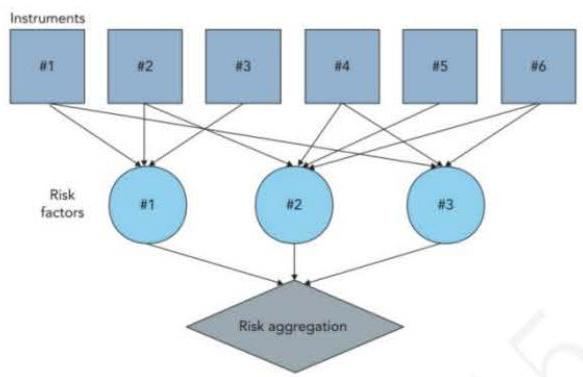
\includegraphics[width=0.4\textwidth]{images/RISKAGGRESION.jpg}
    \end{center}
    \hspace*{3em} 
    
    \begin{itemize}
    \item The principles for VaR risk mapping are summarized as follows:
    \end{itemize}
    
    V VaR mapping aggregates risk exposure when it is impractical to consider each position separately. 【在无法单独考虑每个头寸时， VaR 映射将风险敞口进行聚合。例如，可能需要太多的计算来测量每个单独头寸的风险。】
    
    VaR mapping simplifies risk exposures into primitive risk factors. 【VaR 映射将风险敞口简化为基本的风险因素】
    
    VaR risk measurements can differ from pricing methods where prices cannot be aggregated.
    
    V VaR mapping is useful for measuring changes over time， as with bonds or options. For example， as bonds mature， risk exposure can be mapped to spot yields that reflect the current position. 【VaR 映射对于随时间变化的情况非常有用， 例如债券或期权。例如， 随着债券到期， 风险敞口可以映射到反映当前情况的即期收益率上。】
    
    VaR mapping is useful when historical data is not available. 【在历史数据不可用时， VaR 映射非常有用】
    
General and Specific Risk
    
    \begin{itemize}
    \item 风险因子的选择需要权衡。the trade-off between better quality of the approximation and faster processing.
    \end{itemize}
    
    More factors lead to tighter risk measurement but also require more time devoted to the modeling process and risk computation.
    
     一般风险 (General Risk) 指的是投资组合面临的与整体市场相关的风险， 这些风险通常是由市场因素造成的， 例如市场波动、行业变化、经济周期等。这其实就是我们一级学习的系统性风险
    
    特定风险(Specific Risk)指的是投资组合面临的与个别资产或头寸相关的风险，这些风险与特定的公司、行业或事件有关，而不是整体市场的波动。 这其实就是一级学习的非系统性风险。
    



    \subsubsection{    2. 映射主要内容    }


    \begin{itemize}
    \item Mapping Fixed-income Portfolios
    \end{itemize}
    
    本金映射 (principal mapping)
    
     久期映射 (duration mapping)
    
     现金流映射 (cash flow mapping)
    
    这个知识需要重点掌握
    
    \begin{itemize}
    \item Mapping Linear Derivatives
    \end{itemize}
    
     Forward Contracts
    
     Commodity Forwards
    
    Forward Rate Agreements

     Interest-Rate Swaps
    
    \begin{itemize}
    \item Mapping Options
    \end{itemize}
    
    (1) Mapping Fixed-income Portfolios
    
    \begin{itemize}
    \item 本金映射 principal mapping
    \end{itemize}
    
    \begin{itemize}
    \item With principal mapping， one risk factor is chosen that corresponds to the average portfolio maturity.
    \end{itemize}
    
     只考虑本金的赎回，只有与债券到期时的本金赎回相关的风险被映射。
    
    \begin{itemize}
    \item 久期映射 duration mapping
    \end{itemize}
    
     With duration mapping， one risk factor is chosen that corresponds to the portfolio duration.
    
     利用久期映射，所选择的风险因子要与组合的久期相符。
    
    \begin{itemize}
    \item 现金流映射 cash flow mapping
    \end{itemize}
    
    With cash-flow mapping， the portfolio cash flows are grouped into maturity buckets.
    
     通过现金流映射，将投资组合现金流按照期限进行分组。
    
    \begin{itemize}
    \item 原版书例子: 【这里例子很重要， 一定要读懂。表格中的数据， 重点关注红色字体的。其他数据， 是原版书没有给出来源， 而且对于 mapping 的理解没有那么重要】
    \end{itemize}
    
    a two-bond portfolio consisting of a USD 100 million 5-year 6 percent issue and a USD 100 million 1-year 4 percent issue. Both issues are selling at par， implying a market value of USD 200 million.The portfolio has an average maturity of 3 years and a duration of 2.733 years. The table lays out the present value of all portfolio cash flows discounted at the appropriate zero-coupon rate.
    
    用三种映射求这个债券组合的 VaR。
    
    \begin{center}
    \adjustbox{max width=\textwidth}{
    \begin{tabular}{|c|c|c|c|c|c|c|}
    \hline
    \multirow{2}{*}{Term (Year)} & \multicolumn{2}{|c|}{Cash Flows} & \multirow{2}{*}{Spot Rate} & \multicolumn{3}{|c|}{Mapping (PV)} \\
    \cline{2-3}
    \cline{5-7}
     & 5 年期债券 & 1 年期债券 &  & Principal & Duration & Cash Flow \\
    \cline{1-7}
    1 & 6 & 104 & 4.000\% & 0.00 & 0.00 & 105.77 \\
    \cline{1-7}
    2 & 6 & 0 & 4.618\% & 0.00 & 0.00 & 5.48 \\
    \cline{1-7}
    2.733 & - & - & \phantom{X} & - & 200.00 & - \\
    \cline{1-7}
    3 & 6 & 0 & 5.192\% & 200.00 & 0.00 & 5.15 \\
    \cline{1-7}
    4 & 6 & 0 & 5.716\% & 0.00 & 0.00 & 4.80 \\
    \cline{1-7}
    5 & 106 & 0 & 6.112\% & 0.00 & 0.00 & 78.79 \\
    \cline{1-7}
    总计 & \phantom{X} & \phantom{X} & \phantom{X} & 200.00 & 200.00 & 200.00 \\
    \cline{1-7}
    \hline
    \end{tabular}
    }
    \end{center}
    
    \begin{center}
    \adjustbox{max width=\textwidth}{
    \begin{tabular}{|c|c|c|c|c|c|c|}
    \hline
    Term (Year) & 现金流 & 折现因子 & 旧现金流的 现值 & Risk (\%) & 折现因子 & 新现金流的 现值 \\
    \cline{1-7}
    1 & 110 & 0.9615 & 105.77 & 0.4696 & 0.9570 & 105.27 \\
    \cline{1-7}
    2 & 6 & 0.9136 & 5.48 & 0.9868 & 0.9046 & 5.43 \\
    \cline{1-7}
    3 & 6 & 0.8591 & 5.15 & 1.4841 & 0.8463 & 5.08 \\
    \cline{1-7}
    4 & 6 & 0.8006 & 4.80 & 1.9714 & 0.7848 & 4.71 \\
    \cline{1-7}
    5 & 106 & 0.7433 & 78.79 & 2.4261 & 0.7252 & 76.87 \\
    \cline{1-7}
    \hline
    \end{tabular}
    }
    \end{center}
    
    【1 年期的 VaR=0.4696\%，2 年期的 VaR=0.9868\%，3 年期的 VaR=1.4841\%，4 年期的 \(\mathrm{{VaR}} = {1.9714}\% ，5\) 年期的 \(\mathrm{{VaR}} = {2.4261}\%  \)】
    
    \begin{itemize}
    \item 具体过程:
    \end{itemize}
    
     Principal mapping considers the timing of redemption payments only.
    
     映射时只考虑本金赎回时间，不考虑票面利息。
    
     只有两笔本金: 一个到期时间 5 年， 一个到期时间 1 年。那么这个债券组合平均到期时间是 3 年。
    
     把这个债券组合， 映射到一个到期时间是 3 年的零息债券。而 3 年期的 VaR=1.4841\%
    
    所以，组合的 \(\mathrm{{VaR}} = {200}^{ * }{1.4841}\%  = {2.97}\)
    
     优缺点: 优点: 简单
    
    缺点: This approach overstates the true risk because it ignores intervening coupon payments. 【高估风险】
    
    \begin{itemize}
    \item duration mapping
    \end{itemize}
    
     计算出这个债券组合的麦考林久期。
    
     债券组合的麦考林久期是 2.733 年。【如果题目没给，需要利用一级的方法把麦考林久期计算出来】
    
    3 把这个债券组合映射成一个到期时间是 2.733 年的零息债券。但是题目没有给出 2.733 年的零息债券的 VaR，需要我们利用线性插值法求出:
    
    \({\mathrm{{VaR}}}_{2.733} = {0.987}\%  + \left( {{1.484}\%  - {0.987}\% }\right)  \times  \left( {{2.733} - 2}\right)  = {1.351}\%\)
    
     因此，组合的 \(\mathrm{{VaR}} = {1.351}\%  \times  {200} = {2.7}\)
    
     优点: 比 Principal mapping 稍微精确点。
    
    Cash flow mapping
    
     the cash-flow mapping method consists of grouping all cash flows on term-structure "vertices" that correspond to maturities for which volatilities are provided. 【也就是每个到期期限的现金流， 都映射成一
    
    个零息债券】
    
    \begin{center}
    \adjustbox{max width=\textwidth}{
    \begin{tabular}{|c|c|c|c|c|c|c|c|c|}
    \hline
    \multirow{2}{*}{Term (Year)} & PV Cash Flows & Individual VaR & \multicolumn{5}{|c|}{Correlation Matrix R} & Component VaR \\
    \cline{2-9}
     & \(x\) & xV & 1 年 & 2 年 & 3 年 & 4 年 & 5 年 & xΔVaR \\
    \cline{1-9}
    1 & 105.77 & 0.4966 & 1 & \phantom{X} & \phantom{X} & \phantom{X} & \phantom{X} & 0.45 \\
    \cline{1-9}
    2 & 5.48 & 0.0540 & 0.897 & 1 & \phantom{X} & \phantom{X} & \phantom{X} & 0.05 \\
    \cline{1-9}
    3 & 5.15 & 0.0765 & 0.886 & 0.991 & 1 & \phantom{X} & \phantom{X} & 0.08 \\
    \cline{1-9}
    4 & 4.80 & 0.0947 & 0.866 & 0.976 & 0.9940 & 1 & \phantom{X} & 0.09 \\
    \cline{1-9}
    5 & 78.79 & 1.9115 & 0.855 & 0.966 & 0.9880 & 0.998 & 1 & 1.90 \\
    \cline{1-9}
    总计 & 200.00 & 2.6335 & \multicolumn{6}{|c|}{\phantom{X}} \\
    \cline{1-9}
    \multicolumn{2}{|c|}{Undiversified VaR} & 2.63 & \multicolumn{6}{|c|}{\phantom{X}} \\
    \cline{1-9}
    \multicolumn{2}{|c|}{Diversified VaR} & \multicolumn{6}{|c|}{\phantom{X}} & 2.57 \\
    \cline{1-9}
    \hline
    \end{tabular}
    }
    \end{center}
    
    【Correlation Matrix 相关性矩阵， 两两资产的相关系数， 用来计算组合 diversified VaR。比如 0.897 ， 表示 1 年的现金流和 2 年的现金流相关性是 0.897 】
    
     把组合中的 5 笔现金流， 分别映射成对应期限的零息债券。
    
     在求组合 \(\mathrm{{VaR}}\) 的过程中: 根据资产之间的相关性，可以分为 Undiversified VaR 和 Diversified VaR【关于这个知识点， 在二级《风险管理和投资管理》科目中会详细介绍】
    
    简单说来: Undiversified VaR 认为资产之间的相关系数为 1 ， 也就是完全正相关。没有风险分散化效果
    
    Diversified VaR 资产之间的相关系数小于 1 ， 有分散化效果。
    
    \(>\) Undiversified \(\operatorname{VaR} = {0.4966} + {0.0540} + {0.0765} + {0.0947} + {1.9115} = {2.63}\)
    
    Diversified \(\mathrm{{VaR}} = {2.57}\)
    
    \(>\) 现金流映射方法是最复杂、耗时最多的方法，得来的 VaR 也是最精确的。
    
    \begin{itemize}
    \item Tracking error VaR
    \end{itemize}
    
    \begin{itemize}
    \item Tracking error VaR: the VaR of the deviation between the target portfolio and the benchmark portfolio.
    \end{itemize}
    
     可以用来评估投资组合管理的有效性和相对表现。
    
    Minimizing absolute market risk is not the same as minimizing relative
    
    market risk.
    
    \begin{center}
    \adjustbox{max width=\textwidth}{
    \begin{tabular}{|c|c|c|c|c|c|c|c|}
    \hline
    \multicolumn{3}{|c|}{\phantom{X}} & \multicolumn{5}{|c|}{Position: Portfolio} \\
    \cline{1-8}
    Vertex & Risk (\%) & Position: Index (USD) & 1 (USD) & 2 (USD) & 3 (USD) & 4 (USD) & 5 (USD) \\
    \cline{1-8}
    ≤1m & 0.022 & 1.05 & 0.0 & 0.0 & 0.0 & 0.0 & 84.8 \\
    \cline{1-8}
    \(3\mathrm{\;m}\) & 0.065 & 1.35 & 0.0 & 0.0 & 0.0 & 0.0 & 0.0 \\
    \cline{1-8}
    6m & 0.163 & 2.49 & 0.0 & 0.0 & 0.0 & 0.0 & 0.0 \\
    \cline{1-8}
    1Y & 0.470 & 13.96 & 0.0 & 0.0 & 0.0 & 59.8 & 0.0 \\
    \cline{1-8}
    2Y & 0.987 & 24.83 & 0.0 & 0.0 & 62.6 & 0.0 & 0.0 \\
    \cline{1-8}
    3Y & 1.484 & 15.40 & 0.0 & 59.5 & 0.0 & 0.0 & 0.0 \\
    \cline{1-8}
    4Y & 1.971 & 11.57 & 38.0 & 0.0 & 0.0 & 0.0 & 0.0 \\
    \cline{1-8}
    5Y & 2.426 & 7.62 & 62.0 & 0.0 & 0.0 & 0.0 & 0.0 \\
    \cline{1-8}
    7Y & 3.192 & 6.43 & 0.0 & 40.5 & 0.0 & 0.0 & 0.0 \\
    \cline{1-8}
    9Y & 3.913 & 4.51 & 0.0 & 0.0 & 37.4 & 0.0 & 0.0 \\
    \cline{1-8}
    10Y & 4.250 & 3.34 & 0.0 & 0.0 & 0.0 & 40.2 & 0.0 \\
    \cline{1-8}
    15Y & 6.234 & 3.00 & 0.0 & 0.0 & 0.0 & 0.0 & 0.0 \\
    \cline{1-8}
    20Y & 8.146 & 3.15 & 0.0 & 0.0 & 0.0 & 0.0 & 0.0 \\
    \cline{1-8}
    30Y & 11.119 & 1.31 & 0.0 & 0.0 & 0.0 & 0.0 & 15.2 \\
    \cline{1-8}
    Total & \phantom{X} & 100.00 & 100.0 & 100.0 & 100.0 & 100.0 & 100.0 \\
    \cline{1-8}
    Duration & \phantom{X} & 4.62 & 4.62 & 4.62 & 4.62 & 4.62 & 4.62 \\
    \cline{1-8}
    Absolute VaR & \phantom{X} & USD 1.99 & USD 2.25 & USD 2.16 & USD 2.04 & USD 1.94 & USD 1.71 \\
    \cline{1-8}
    Tracking error VaR & \phantom{X} & USD 0.00 & USD 0.43 & USD 0.29 & USD 0.16 & USD 0.20 & USD 0.81 \\
    \cline{1-8}
    \hline
    \end{tabular}
    }
    \end{center}
    
    【第三个组合的 Tracking error VaR，最小， 是 0.16。其大部分权重配置在了 2 年期的债券， 这和 index 的配置权重(其最大的权重 24.83， 也配置在了 2 年期的债券)最接近 】
    
    (2) Mapping Linear Derivatives
    
     原则:看这种衍生品构成的要素。
    
     Forward Contracts 【主要是外汇远期】
    
    \[
    {\mathrm{F}}_{\mathrm{t}} = \left( {{\mathrm{S}}_{\mathrm{t}}{\mathrm{e}}^{-\mathrm{{yt}}}}\right) {\mathrm{e}}^{\mathrm{{rt}}}
    \]
    
    \(\mathrm{r}\) 是本币的无风险利率； \(\mathrm{y}\) 是外币的无风险利率。
    
    买入外汇远期， 等价于买入外汇现货， 同时买入外币短期国债， 卖出本币短期国债。
    
    若要计算外汇远期的 VaR， 只需要分别计算出现货、外币短期国债和本币短期国债的 VaR。若计算 Undiversified VaR，几个 VaR 直接相加即可; 若计算 Diversified VaR，还要考虑资产之间的相关性。
    
    Forward Rate Agreements (FRA)
    
    Long 6 × 12 FRA=long 6-month bill + short 12-month bill
    
    This is equivalent to borrowing USD 100 million for 12 months and investing the proceeds for 6 months
    
    Short 6 \(\times  {12}\) FRA= short 6-month bill+ long 12-month bill
    
    This is equivalent to borrowing USD 100 million for 6 months and investing the proceeds for 12 months
    
    Interest-rate swaps
    
    利率互换有两种拆分: 拆分为固定利率、浮动利率债券， 和一系列的远期合约
    
    一种: A swap with receiving floating rate and paying fixed rate=long floating-rate bond + short fixed-rate bond
    
    另一种: A portfolio of forward contracts.
    
    (3) Mapping Options
    
     这里主要是欧式期权
    
    BSM model(看涨期权)
    
    \[
    \mathrm{c} = {\mathrm{{Se}}}^{-\mathrm{{yt}}}\mathrm{N}\left( {\mathrm{d}}_{1}\right)  - {\mathrm{{Ke}}}^{-\mathrm{{rt}}}\mathrm{N}\left( {\mathrm{d}}_{2}\right)
    \]
    
    Long call option \(=\) long \(\bigtriangleup\) asset+ short \(\left( {\bigtriangleup \mathrm{S} - \mathrm{c}}\right)\) bill
    
    \(\mathrm{N}\left( {\mathrm{d}}_{1}\right)  = \Delta\)
    
    \({\mathrm{{Ke}}}^{-\mathrm{{rt}}}\mathrm{N}\left( {\mathrm{d}}_{2}\right)  = \mathrm{{SN}}\left( {\mathrm{d}}_{1}\right)  - \mathrm{c} = \bigtriangleup \mathrm{S} - \mathrm{c}\)
    




\subsection{验证银行控股公司的风险价值模型}

\begin{itemize}
    
    \item 巴塞尔委员会1996 年规定用VaR 模型计算银行资本， VaR 模型要进行回测。
美国银行机构还要求进行概念合理性(conceptual soundness) 、结果分析和基
准测试等。【2025 年新增】
\item 小概念： pseudo history（伪历史数据）
在VaR 模型构建过程中， 需要历史数据来进行分析和模型估计。由于
实际情况的复杂性， 真实的历史数据不可得或者不能直接使用。通过一
定的方法和假设构建出来的类似历史数据的数据， 就被称为pseudo
history 。
\end{itemize}

\subsubsection{Conceptual Soundness}
银行的模型验证指南要求审查VaR 模型的概念合理性。【通俗地来说， 概念合
理性就是说一个模型在最基本的理念和设计上要站得住脚】

The banking guidance on model validation requires a review of conceptualsoundness of the model.
    \begin{itemize}
    \item (1) 确定模型所使用的假设、技术和数据是否恰当This requires the validator to determine whether the model assumptions， techniques and data used are appropriate.
        \begin{itemize}
        \item In most cases this is accomplished through a narrative provided by the validator. 通常通过验证者提供的说明来完成
        \end{itemize}
    \item (2) A very basic decision: whether the model is suitable for the purpose it is developed for. 【模型应符合其开发目的】
        \begin{itemize}
        \item VaR 模型的关键目的： 帮助公司管理头寸的风险当头寸变化时， 风险如何变化
            \begin{itemize}
            \item In the case of VaR models，their basic purpose is to help the firm manage the risk of its positions; its key purpose is to show how risk changes when positions change. VaR models that cannot be used to show how risk changes when positions change are not "fit for purpose" and thus fail a crucial conceptual soundness test in the model validation process. 【不能展示头寸风险变化的模型不是“ 好模型”， 即无法通过crucial conceptual soundness test】
            \end{itemize}
        \item they have other uses such as for capital calculations， but these are perhaps ancillary（辅助） to the risk management purpose.
            \begin{itemize}
            \item 【VaR 模型的辅助功能比如资本计算 没那么重要】
            \end{itemize}
        \end{itemize}
    \item (3) 还可运用敏感性分析sensitivity analysi s 等定量测试quantitative tests 。有助于评估模型性能、数据问题及估计误差的严重程度。【关千敏感性分析sensitivity analysis 详见后面知识点】
        \begin{itemize}
         \item Beyond the consideration of how the model will be used， the conceptual soundness of the model can be considered using more quantitative test s.
        These include sensitivity analysis that can show the effect of data limitations or choices and provide statistical confidence intervals around VaR estimates.
        These can answer fundamental questions regarding the per formance of the VaR model and can also assess the severity of data problems and estimation errors.
        \end{itemize}
    \end{itemize}

\subsubsection{VaR 模型的sensitivity analysis}
\textbf{方式 1: 分解和基于回归的方法:}

\begin{itemize}
    \item Value-at-Risk 是线性齐次的（线性齐次性）在头寸上。因此满足欧拉方程：
    \[
    VaR_{PT} = \sum_{i \in P} \frac{\partial VaR_{p}}{\partial v_{iT}} * v_{iT} = \sum_{i \in P} MVaR_{iT} * v_{iT}
    \]
    \item 与 \( \Delta v_i \) 的回归关系，可以得到下面这个公式：
    \[
    CVaR_{i} = VaR_{p} * \omega_{i} * \beta_{i，p}
    \]
    \begin{itemize}
        \item \( i \): 投资组合中的单个资产
        \item \( P \): 投资组合
        \item \( T \): 时间
        \item \( \omega_{i} \): 资产 \( i \) 在组合中的权重
        \item \( \beta_{i，p} \): 资产 \( i \) 对于整体投资组合价值的敏感程度
        \item \( \frac{\partial VaR_{p}}{\partial v_{i}} = MVaR_{i} \): 边际 VaR
        \item \( CVaR_{i} \): 成分 VaR
    \end{itemize}
    \item 关于 VaR 和成分 VaR 更详细的，见《Risk Management and Investment Management》的“Chapter 5 Portfolio Risk”部分。
\end{itemize}

\textbf{某些特定头寸的风险，与 \( \omega_{i} \) 和 \( \beta_{i，p} \) 是相关的。通过敏感性分析可以明确 VaR 会如何随着这些参数的变化而变化。}

\begin{itemize}
    \item 如果金融机构对其在某个特定头寸的估值所做的选择有担忧，这种分析可以帮助说明 VaR 是多么敏感于估值选择。
    \item 问题：难以获得合适的数据。因为这需要完整的时间序列来反映头寸的变化值。
\end{itemize}

\textbf{方式 2: 替代方案}

由 Tasche (2000) 和 Hallerbach (2003) 提出，主要适用于方式 1 回归方法不可行时的替代，并且该方法适用于其历史模型法。

Tasche 和 Hollerbach 表明线性齐次性意味着：
\[
VaR_{PT} = \Delta V^*_{PT} = \sum_{i \in P} E(\Delta V_{iT} | \Delta V_{PT}) = \Delta V^*_{PT}
\]

\begin{itemize}
    \item \( \Delta V^*: \) 代表投资组合在某一特定情景下的价值变化量。
    \item \( \sum_{i \in P} E(\Delta V_{iT} | \Delta V_{PT}) \): 表示对投资组合中每个头寸的价值变化 \( \Delta V_{iT} \) 的期望。
\end{itemize}

简言之：投资组合的风险价值 \( VaR_{PT} \) 等同于在特定情景 \( \Delta V_{PT} \) 下，投资组合内各个头寸对价值变化的条件期望。

\begin{itemize}
    \item 每个头寸的成分 VaR 可以通过在确定情景下每个头寸可能经历的价值变化来估计。
    \item 若数据缺失 \(\rightarrow\) 简化处理: In the case of a "missing" position this reduces the problem of estimating the component VaR to observing how much it would have lost on the day that determines the VaR. 【若数据缺失，想获得成分 VaR，可简化为仅观察该缺失头寸在确定组合 VaR 的那一天可能遭受的损失金额】

    \item 简化处理未必可靠 \(\rightarrow\) 改进: This single observation is less reliable than an estimate based on multiple observations， so the average of the ordered observations near the HS-VAR may be used instead. 【要提高 VaR 的可靠性，需要寻找接近 HS - VAR 的平均值。例如，找到与缺失数据类似的头寸，在相似市场条件下，获得其价值变化数据，得出这些数据的 VaR， 取其平均作为缺失数据的头寸的 VaR】
    
\end{itemize}

\textbf{敏感性分析}

\begin{itemize}
    \item 风险评估：敏感性分析有助于理解个别头寸如何影响整体 VaR。
    \item 风险管理：根据敏感性结果，企业可以决定是否增加或减少对某些资产或头寸的敞口。
    \item 模型评估：有助于评估模型的假设和简化。
\end{itemize}

\textbf{敏感性分析挑战：}

\begin{itemize}
    \item 数据稀缺：可能得出不准确的敏感性分析结果。
    \item 投资组合的复杂性：实际上，投资组合可能非常复杂且变化迅速。此外， 不同头寸之间的相关性也可能随时间变化，都增加了分析的复杂性。
\end{itemize}

\subsubsection{VaR 的置信区间confidence intervals}

3. VaR 的置信区间 confidence intervals

\begin{itemize}
\item 背景知识:
\end{itemize}

 在估计组合 VaR 时， 人们会关注准确性。从统计学角度， 可通过置信区间来解决，使 VaR 真实值在概率上会落在该区间内。

\(\rightarrow\) 一级时，我们学过置信区间的计算: \(\left\lbrack  {\widehat{\mu } - {\mathrm{C}}_{\alpha } \times  \frac{\widehat{\sigma }}{\sqrt{\mathrm{n}}}，\widehat{\mu } + {\mathrm{C}}_{\alpha } \times  \frac{\widehat{\sigma }}{\sqrt{\mathrm{n}}}}\right\rbrack\)

\begin{itemize}
\item \(\frac{\widehat{\sigma }}{\sqrt{n}}\) : 标准误
\end{itemize}

这里给出了特定的标准误-asymptotic standard error:

\[
\operatorname{SE}\left( {\operatorname{VaR}}_{\mathrm{{PT}}}^{1 - c}\right)  = \sqrt{\frac{c\left( {1 - c}\right) }{T * f{\left( {\operatorname{VaR}}_{\mathrm{{PT}}}^{1 - c}\right) }^{2}}}
\]

c:coverage level 通常等同于 confidence level 置信水平

f(   ):VaR 的概率密度函数 probability density function

\({\mathrm{C}}_{\alpha }\) 是变量服从某个分布对应的关键值

 在计算置信区间会面临很多挑战， 比如数据的质量和数量、组合的复杂性和相关性变化， 计算强度等。更重要的是确定 VaR 服从的分布， 即 VaR 的概率密度函数 probability density function。

\begin{itemize}
\item 概率密度函数难题
\end{itemize}

 在确定 VaR 的概率密度函数时， 通常假设其是服从正态分布的， 但是金融收益通常非正态分布， 采用正态分布假设会出错。

it is a stylized fact that financial returns are non-normal so imposing a normal distribution would probably be a mistake.

 确定 VaR 的真实概率密度函数并非易事。不同投资组合可能有不同的潜在分布， 精准识别并运用正确的分布是个挑战。

\begin{itemize}
\item 基于不同方法计算 VaR 置信区间
\end{itemize}

 Two approaches in the academic literature are the use of order statistics (Dowd 2006) or the use of bootstrap techniques Christoffersen and Goncalves 2006).

 Order statistics 顺序统计量方法

大致逻辑:

(1)先对投资组合伪历史数据 pseudo history 排序，

(2)利用特定公式计算概率

\[
\text{ 特定公式: }\;{G}_{r}\left( {\Delta V}\right)  = \mathop{\sum }\limits_{{j = r}}^{T}\left( \begin{matrix} T \\  j \end{matrix}\right) {\left\lbrack  F\left( \Delta V\right) \right\rbrack  }^{j}{\left\lbrack  1 - F\left( \Delta V\right) \right\rbrack  }^{n - j}
\]

\(\mathrm{F}\left( {\Delta \mathrm{V}}\right)\) : 组合价值变化观测值的累积密度函数

( 3 )通过设置不同概率值(如 0.05 和 0.95 对应 90\%置信区间)，并求解得到下限和上限对应的函数值

(4)再依据不同的 VaR 模型(如历史模拟 VaR、GARCH 模型)进一步确定具体的置信区间取值。

bootstrap 自助法

(1) 针对历史模拟 VAR 的置信区间计算: it does assume independence of the changes in portfolio value over time and thus does not reflect possible dependence in returns over time.【这种方法没有考虑相关性】。

大致流程如下:

从伪历史数据中有放回地取样 replacement， 计算 VaR

多次重复上述过程，可计算多个 VaR 值

用抽样分布中特定百分位数确定置信区间

(2) 针对 GARCH VaR 的置信区间计算: The GARCH VaR accounts for the dependence of changes in portfolio values. 【考虑了相关性】 大致流程如下:

从独立同分布 (IID) 序列重抽样生成自助样本 bootstrap sample。

用自助样本重新估计 GARCH 模型参数， 得到新的波动率等值。

根据新的估计值和相关公式计算 GARCH VaR

重复上述步骤多次 (如 B 次)， 得到的 B 个 VaR

给定置信水平 CI，通过计算排序后的 VaR 值确定置信区间。

(3) 针对 Filtered Historic Simulation 滤波历史模拟模型的置信区间计算: 重新估计残差，并依据相应方程为每个样本重新计算 \(\mathrm{{VaR}}\) ，进而计算置信区间。

 Empirical likelihood 经验似然方法: 除了上面 order statistics 和 bootstrap techniques 两种， 原版书在这里还提出了 Empirical likelihood 方法。有学者针对不同模型(如 Chan 等人针对 GARCH 模型、Gong Li 和 Peng 针对 ARCH 模型)提出用经验似然为 VaR 模型计算置信区间。 【简单了解】

结果:

通过计算标普 500 (S\&P 500) 收益率 1 天 99\% VaR 的置信区间， 不同 VaR 计算方法(历史模拟、GARCH、过滤历史模拟)及不同计算置信区间方法，发现:

(1)置信区间通常不对称(confidence intervals are not symmetric)，且估计 VaR 的数据越多，置信区间越窄(tighter confidence intervals).

(2)历史模拟法中，顺序统计量和自助法计算出的置信区间有差异，但无证据表明哪种更好

(3)在市场压力时期，历史模拟法下的 VaR 具有特别宽的置信区间。

(4)Filtered Historic Simulation 的置信区间较窄，意味着其对 VaR 的估计更有效。Most notable are the narrow confidence intervals for filtered historic

simulation， suggesting that it provides more efficient estimates of VaR

【置信区间窄， 意味着精确度更高】

\begin{center}
\adjustbox {max width=\textwidth}{
\begin{tabular}{|c|c|c|c|c|c|c|c|c|}
\hline
VaR method & Cl method & \(\mathrm{N}\) & Date range & VaR & \multicolumn{2}{|c|}{95\% Cl} & \multicolumn{2}{|c|}{\(\mathrm{{Cl}}\) as a percentage of VAR} \\
\cline{1-9}
HS & Bootstrap & 250 & 5/2016-5/2017 & 1.725 & 1.347 & 1.98 & 21.9 & 14.8 \\
\cline{1-9}
HS & Bootstrap & 9424 & 1/1980-5/2017 & 2.878 & 2.727 & 3.138 & 5.2 & 9.0 \\
\cline{1-9}
HS & Bootstrap & 253 & \(8/{2008} - 8/{2009}\) & 8.439 & 5.536 & 10.58 & 34.4 & 25.4 \\
\cline{1-9}
HS & Bootstrap & 755 & 8/2006-8/2009 & 5.662 & 4.103 & 6.271 & 27.5 & 10.8 \\
\cline{1-9}
HS & Order & 250 & 5/2016-5/2017 & 1.725 & 1.358 & 1.761 & 21.3 & 2.1 \\
\cline{1-9}
HS & Order & 9424 & 1/19 80-5/2017 & 2.878 & 2.729 & 3.137 & 5.2 & 9.0 \\
\cline{1-9}
HS & Order & 253 & 8/2008-8/2009 & 8.439 & 5.008 & 10.24 & 40.7 & 21.3 \\
\cline{1-9}
HS & Order & 755 & 8/2006-8/2009 & 5.662 & 4.001 & 6.171 & 29.3 & 9.0 \\
\cline{1-9}
Garch & Order & 250 & 5/2016-5/2017 & 1.109 & 0.846 & 1.152 & 23.7 & 3.9 \\
\cline{1-9}
Garch & Order & 9424 & 1/19 80-5/2017 & 1.11 & 0.903 & 1.252 & 18.6 & 12.8 \\
\cline{1-9}
Garch & Order & 253 & 8/2008-8/2009 & 2.91 & 2.443 & 3.3 & 16.0 & 13.4 \\
\cline{1-9}
Garch & Order & 755 & 8/2006-8/2009 & 2.815 & 2.579 & 3.101 & 8.4 & 10.2 \\
\cline{1-9}
FHS & Order & 250 & 5/2016-5/2017 & 1.205 & 1.188 & 1.222 & 1.4 & 1.4 \\
\cline{1-9}
FHS & Order & 9424 & 1/19 80-5/2017 & 1.324 & 1.314 & 1.334 & 0.8 & 0.8 \\
\cline{1-9}
FHS & Order & 253 & 8/2008-8/2009 & 3.109 & 3.001 & 3.136 & 3.5 & 0.9 \\
\cline{1-9}
FHS & Order & 755 & 8/2006-8/2009 & 3.239 & 3.158 & 3.284 & 2.5 & 1.4 \\
\cline{1-9}
\hline
\end{tabular}
}
\end{center}


\subsubsection{Benchmarking VaR models} 

\begin{itemize}
\item Benchmarking VaR models 是指对 VaR 模型进行基准测试的过程。
\end{itemize}

 目的在于将银行所使用的 VaR 模型与其他替代模型进行比较， 进而评估该模型的性能优劣与有效性。

\begin{itemize}
\item 挑战及克服方法:
\end{itemize}

【在 VaR 模型进行基准测试时存在挑战及相应的解决方法】

 第一个挑战: 交易组合频繁变动， 导致误差非独立同分布。The first is that trading portfolios change frequently so that errors are not independent and identically distributed.

【背景知识:传统的统计模型和金融模型， 如线性回归模型、时间序列模型等， 在进行参数估计和推断时， 通常都假设数据是独立同分布的。这是因为在这些假设下， 可以利用中心极限定理等数学工具来推导模型的性质和统计检验。例如， 在普通最小二乘法 (OLS) 回归中， 假设误差项是独立同分布的正态分布。如果数据不满足独立同分布假设， 这些传统的理论和方法就需要进行调整或采用其他方法来处理数据。】

克服方法: Christoffersen et al. (2001) propose methods to overcome this but restrict this to distributions that are location scale models 位置尺度模型 so that the quantile is a linear function of the volatility. 【使用特定的分布模型(即 location scale models)。在这种模型中， 分位数和波动率存在线性关系。】

 第二个挑战: 缺乏可用模型。The second aspect is that banks rarely have two VaR models available to compare。银行构建一个单一的 VaR 模型就已经很耗时耗力。构建两个模型只会使问题更加复杂。

克服方法:基于交易利润和损失的 GARCH (1，1) VaR 模型: Berkowitz and O'Brien (2002) overcome this issue by estimating a GARCH(1，1)VaR model on the profit and loss from trading by the bank.基于交易利润和损失的 GARCH (1，1) VaR 模型， 虽然可能不适合银行风险管理，但可用于对比，且具有一定的参考价值。


\subsection{Beyond Exceedance-Based Backtesting of VaR Models(超越超出基于VaR模型的回测)}    


这个 chapter 是对于前面 chapter-Backtesting VaR 的补充和深化. 【2025 年新内容， 和回测有关所以放在了 Backtesting VaR 后面】

Backtesting VaR 主要涉及关于传统的回测方法; 这个 chapter 提出 PIT 方法， 为 VaR 模型评估提供了一种新的视角和分析手段。


\subsubsection{基本概念}


\begin{itemize}
    \item Exceedance-based backtest: 基于 exceedance 的回测。就是 "Backtesting VaR" 中的回测。
    \end{itemize}
    
    \begin{itemize}
    \item A standard backtesting practice is to count instances when daily P\&L is lower than the ex ante VaR (i.e.， portfolio loss exceeds its estimated VaR).
    \end{itemize}
    
     ex ante VaR: 事前 VaR
    
     理解: 例如， 95\% 置信水平下的 VaR 为 100 万元。如果某一天的实际 P\&L 为 -120 万元(即损失了 120 万元)，表明实际损失突破了 VaR 的估计，出现了一个 exception 情况。
    
     These instances are also known as VaR exceedances， exceptions or breaches.
    

\subsubsection{VaR回测的特性}


\begin{itemize}
    \item According to Christoffersen (1998)， any backtesting of a VaR model that accurately reflects the actual distribution of the P\&L is expected to have two distinct properties:
    \end{itemize}
    
    1) unconditional coverage 无条件覆盖
    
    \begin{itemize}
        \item 由 Kupiec (1995)给出。
    
        \item The unconditional coverage property restricts the number of exceedances which may be observed in a given time period at a determined statistical significance level (again， in the regulatory context， this is a one-day horizon with a \({99}\%\) confidence level). 【unconditional coverage 指的是在特定的显著性水平下， 给定时间范围内， 实际损失超过 VaR (即出现超越情况) 的次数应符合模型预先设定的概率。】
        \begin{itemize}

            \item 例如，在 99\% 置信水平的 VaR 中，理论上应该只有 1\% 的时间会出现实际损失超过 VaR 的情况。若 100 天的 P\&L 数据， 超过 VaR 的损失应该只有 1 个。
        \end{itemize}

    \item Unconditional coverage is analogous( 类 似 ) to the uniformity distributional property of a series of PITs. 【无条件覆盖具有类似于一系列 PIT 的均匀分布特性。】
    \begin{itemize}

        \item 无条件覆盖和 PITs 的均匀分布特性在本质上有相似之处
\end{itemize}

    \(\diamond\) In other words， the series of probabilities of observing each P\&L outcome in relation to VaR should be uniformly distributed over a zero to one interval， \(\mathrm{U}\left( {0，1}\right)\) .
    
    \item 例如，假设一个投资组合的 VaR 在 95\% 置信水平下为 100 万元，那么实际损失小于 100 万元的概率应该接近 95\%，实际损失大于 100 万元的概率接近 5\%。更广泛地来看， 它们相对于 VaR 的出现概率应该像在区间 \(\left\lbrack  {0，1}\right\rbrack\) 上均匀分布，没有明显的聚集或偏差。
    
    补充知识: \(\mathrm{U}\left( {0，1}\right)\) 表示区间 \(\left\lbrack  {0，1}\right\rbrack\) 上的均匀分布 (Uniform Distribution)， 意味着在该区间内的任何一个值被取到的概率是相等的。
    
    \begin{center}
    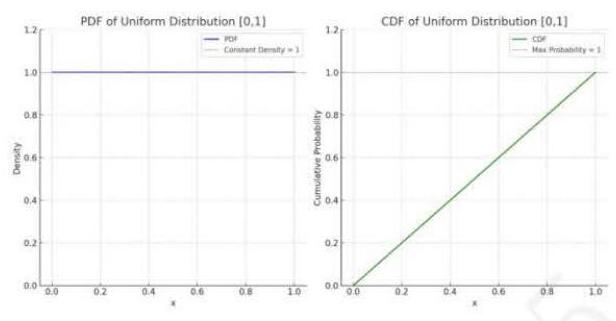
\includegraphics[width=0.5\textwidth]{images/PDFCDF.jpg}
    \end{center}
    \hspace*{3em} 
    

\end{itemize}

    2) independence 独立
    \begin{itemize}

    \item The independence property asserts that the observed exceedances should be independent from one another， and each observed exceedance should not be informative of future exceedances. 【出现 exceedances 次数应该是独立的】
    
    \item Operationally， if a risk model is perfectly accurate， a series of PITs are i.i.d. \(\mathrm{U}\left( {0，1}\right)\) .【i.i.d. \(\mathrm{U}\left( {0，1}\right)\) : 独立同分布的均匀分布 \(\mathrm{U}\left( {0，1}\right)\) 】
    
    \begin{itemize}
    \item Misspecification
    \end{itemize}
    

   
   



    \item 如果偏离上面两个特征， 模型就会出现设定错误 Misspecification:
    
    Conservative misspecification 保守型设定错误: implies that the model distribution is too wide， and P\&L observed is small， clustering in the middle of the distribution (i.e.， the model parameters are too conservative to accurately model market dynamics). \(\rightarrow\) 风险值设定较低
\end{itemize}

    \begin{itemize}
    \item Aggressive misspecification 激进型设定错误: implies that the model distribution is too narrow and we often see realized P\&L in the tails of the distribution. \(\rightarrow\) 风险值设定较高
    \end{itemize}

\subsubsection{Probability Integral Transform(PIT)概率积分变换}



【补充小概念:概率积分变换 PIT 是指任意连续随机变量可以通过其累积分布函数转换为均匀分布， 或者反过来从均匀分布转换为特定分布. 】

\begin{itemize}
\item often called the "p-value"(p 值)，
\end{itemize}

\begin{itemize}
\item PIT associated with the VaR model P\&L as an integral component of a robust backtesting process.
\end{itemize}

\begin{itemize}
\item The PIT was introduced by Diebold et al. (1998) for backtesting of density forecasts and represents the cumulative probability of observing a loss greater than the current P\&L realization based on the previous day's VaR model forecast.
\end{itemize}

 PIT 代表的是一种累积概率， 即在基于前一天的 VaR 模型预测的基础上， 观察到损失大于当前实际盈亏(P\&L)的累积概率。

\begin{itemize}
\item When PITs are well estimated they provide information on the accuracy of the risk model at any percentile of the forecast distribution.
\end{itemize}

\begin{itemize}
\item VaR 模型 PIT 推导。
\end{itemize}

【核心:在 VaR 模型验证的过程中， 利用 PIT 方法来连接模型的预测分布与实际观测数据， 并通过计算和分析 PIT 值来判断模型的好坏。】

 相比于传统回测， PIT 提供了对整个分布的评估， 而不仅局限于某个分位点的风险。

4 大致步骤:

1) 定义预测分布 \({\mathrm{F}}_{\mathrm{t}}\left( \right)\) : if the risk model produces an accurate daily forecast distribution for the portfolio \(\mathrm{P}\& \mathrm{L}，{\mathrm{F}}_{\mathrm{t}}\left( \right)\)

2) 获取实际的收益值 \({\mathrm{{PL}}}_{\mathrm{t} + 1}\) : observing the daily realization of the portfolio \(\mathrm{P}\& \mathrm{L}\) ， \({\mathrm{{PL}}}_{\mathrm{t} + 1}\) ，

3) 计算 PIT 值: calculate the risk model's probability of observing a loss below the actual \(\mathrm{P}\& \mathrm{L}\) ， known as Probability Integral Transform denoted by \({\mathrm{p}}_{\mathrm{t} + 1}\) ， 同理可得周二到周五的 PIT 值，分别是 \({2.28}\% ，{0.62}\% ，{3.59}\% ，{0.13}\% ，{1.79}\%\)

\[
{\mathrm{p}}_{\mathrm{t} + 1} = {\mathrm{F}}_{\mathrm{t}}\left( {\mathrm{{PL}}}_{\mathrm{t} + 1}\right)
\]

拓展: 简化的例子

\({\mathrm{F}}_{\mathrm{t}}\left( \right)\) : 假设某银行的交易组合模型预测 \(\mathrm{P}\& \mathrm{L}\) 服从均值为 0，标准差为 100000 的正态分布， 每日 VaR 为 99\%置信水平。

\[
\text{ VaR=0+(-2.58)*100，000=-258，000 }
\]

PL \({}_{\mathrm{t} + 1}\) 银行记录了一周的实际损益 \(\mathrm{{PL}}\) 和 \(\mathrm{{VaR}}\) 预测分布。数据如下:

\begin{center}
\adjustbox{max width=\textwidth}{
\begin{tabular}{|c|c|}
\hline
日期 & 实际损益(PL) \\
\cline{1-2}
周一 & -200，000 \\
\cline{1-2}
周二 & -250，000 \\
\cline{1-2}
周三 & -180，000 \\
\cline{1-2}
周四 & -300，000 \\
\cline{1-2}
周五 & -210，000 \\
\cline{1-2}
\hline
\end{tabular}
}
\end{center}

计算 PIT 值:

根据实际损益和预测分布的累积分布函数(CDF)计算 PIT 值:

\[
{\mathrm{p}}_{\mathrm{t} + 1} = {\mathrm{F}}_{\mathrm{t}}\left( {\mathrm{{PL}}}_{\mathrm{t} + 1}\right)
\]

周一: 实际损益-200，000

\[
\text{ 标准化: }\mathrm{Z} = \left( {-{200}，{000} - 0}\right) /{100000} =  - 2
\]

查正态分布表: \({\mathrm{F}}_{\mathrm{t}}\left( {-{200000}}\right)  = \Phi \left( {-2}\right)  = {2.28}\%\)

\begin{itemize}
\item Shape of the distribution of PITs
\end{itemize}

a. 如果 VaR 模型是准确的，则 PIT 值应在 \(\left\lbrack  {0，1}\right\rbrack\) 区间内均匀分布。均匀分布表明模型在所有分位点上均能正确反映实际的损失概率。

 The degree to which actual distribution of PITs differs from uniform may provide information regarding the model's ability to accurately and reliably assess risk of a given portfolio of instruments.

b. 非均匀分布的情况 \(\rightarrow\) 模型可能存在问题

\textbackslash / 集中在分布的中间: PIT 分布呈现“驼峰形状”，中间值较多。

The distorted shape of the distributions indicates that when considered in aggregate， models are fairly conservative in the body of the forecast distribution (i.e.， humped shape).

模型过于保守， 低估了尾部风险， 预测范围过宽

 分布在两端: PIT 分布在两端 (接近 0 或 1)。

模型过于激进， 分布范围过窄， 导致实际损失超出预测的频率增加。

The tails of these risk models are thinner than is required by the realizations of P\&L (i.e.， visible spikes at each end of the distribution).

\begin{center}
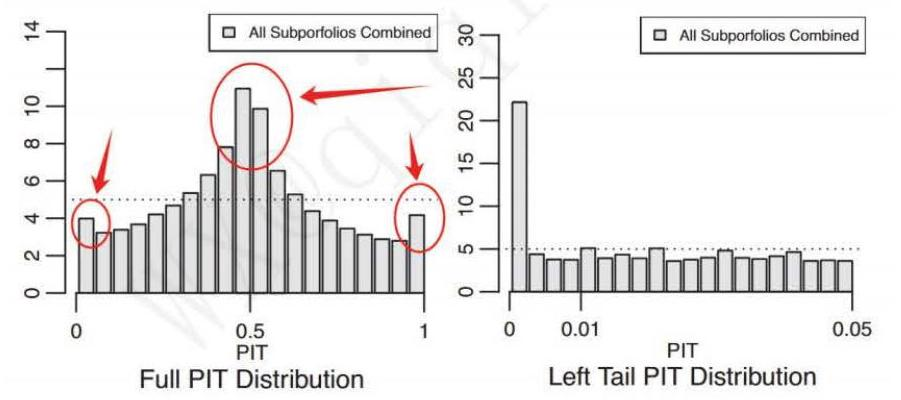
\includegraphics[width=0.7\textwidth]{images/pit.jpg}
\end{center}
\hspace*{3em} 

 偏向分布的一侧: PIT 值集中在靠近 0 或 1 的一侧， 呈现偏移分布。

模型可能存在系统性偏差， 导致高估或低估风险。

VaR models generally produce distributions that overstate variance and understate kurtosis 峰 度. Further， we observe deviations from the expected mean， as well as evidence of skewness 偏度 in either positive or negative direction.


\subsubsection{Goodness-of-fit ests 拟合优度检验}



\begin{itemize}
    \item 运用 Kolmogorov-Smirnov、Anderson-Darling 和 Cramér-von Mises 等检验评估 PIT 分布的均匀性。
    \end{itemize}
    
    (1) Kolmogorov-Smirnov test (KS 检验)
    
     Kolmogorov-Smirnov test (KS) is a widely used nonparametric test that evaluates the goodness-of-fit by comparing the empirical distribution function of a sample with some reference distribution function. 【KS 检验衡量样本分布函数与理论分布函数 (如均匀分布) 之间的最大距离。】
    
    \begin{itemize}
    \item Operationally， the KS statistic quantifies the distance between the empirical CDF of the sample and the CDF of the reference distribution. 【CDF: 累积分布函数】
    \end{itemize}
    
     检验过程:
    
    \begin{itemize}
    \item 原假设: \(\mathrm{D} = 0\)
    \end{itemize}
    
    检验统计量:【公式了解】
    
    \[
    D = \mathop{\max }\limits_{j}\left\{  {\operatorname{abs}\left( {{z}_{j} - {A}_{j}}\right) }\right\}
    \]
    
    \({\mathrm{z}}_{\mathrm{j}}\) is the theoretical CDF ; \({\mathrm{A}}_{\mathrm{j}}\) the empirical CDF
    
    优点:
    
    非参数检验(nonparametric test)， 对整体分布的偏离较敏感。
    
    计算简单，适用于广泛的分布类型。
    
     缺点:
    
    对尾部分布的偏差不敏感 lack of sensitivity at the extremes of the distribution。
    
    在小样本中可能缺乏检测能力。
    
    (2) Anderson-Darling test (A-D 检验)
    
    \(>\) Anderson-Darling test (A-D) is a modification of the Kolmogorov-Smirnov test that corrects for this limitation.
    
     Unlike the KS test， A-D puts more weight on the tails of the distribution， yielding more power in the presence of distributional biases. 【A-D 检验在 KS 检验的基础上增加对尾部的权重。】
    
     检验过程:
    
    \begin{itemize}
    \item 原假设: \({\mathrm{A}}^{2} = 0\)
    \end{itemize}
    
    检验统计量: 【公式了解】
    
    \[
    {A}^{2} =  - n - \frac{1}{n}\mathop{\sum }\limits_{{j = 1}}^{n}\left( {{2j} - 1}\right) \left\lbrack  {\log \left( {z}_{j}\right)  + \log \left( {1 - {z}_{-j}}\right) }\right\rbrack
    \]
    
    \(\mathrm{n}\) is the number of observations
    
     优点:
    
    更重视分布尾部的偏差，对极端事件更敏感。
    
    在金融风险管理中更符合 VaR 模型对尾部风险的关注。
    
     缺点:
    
    计算复杂度较高。
    
    在中间分布上的检验能力稍弱。
    
    (3) Cramér-von Mises test(CM 检验)
    
     基于样本分布函数与理论分布函数的平方偏差
    
     Cramér-von Mises test is another variation of the Kolmogorov-Smirnov test. However， rather than using the supremum， it relies on the mean squared deviation of the distribution. 【supremum:上确界。在数学分析中，指的是一个集合的最小上界】
    
     检验过程:
    
    \begin{itemize}
    \item 原假设: \({\mathrm{W}}^{2} = 0\)
    \end{itemize}
    
    检验统计量: 【公式了解】
    
    \[
    {W}^{2} = \mathop{\sum }\limits_{{j = 1}}^{n}{\left\lbrack  {z}_{j} - \left( 2j - 1\right) /2n\right\rbrack  }^{2} + \left( {1/{12n}}\right)
    \]
    
    \$ 优点:
    
    对分布整体偏离均有较好的检测能力， 包括尾部和中间。
    
    平衡了 Kolmogorov-Smirnov 和 Anderson-Darling 的优点。
    
     缺点:
    
    检验力度可能低于 Anderson-Darling 对尾部偏离的检测。
    
    计算复杂性介于 Kolmogorov-Smirnov 与 Anderson-Darling 之间。
    
    Summary:
    
    \begin{center}
    \adjustbox{max width=\textwidth}{
    \begin{tabular}{|c|c|c|c|}
    \hline
    \phantom{X} & 优点 & 缺点 & 适用场景 \\
    \cline{1-4}
    KS 检验 & 简单有效， 适合整体 分布 & 对尾部衡量不敏感 & 快速评估模型的 总体均匀性 \\
    \cline{1-4}
    A-D 检验 & 对尾部偏差敏感 & 对中间分布的检验 能力稍弱 & 关注尾部风险的 场景 \\
    \cline{1-4}
    CM 检验 & 综合性强， 对整体分 布均匀性检测良好 & 对尾部的检验不如 A-D & 全面评估模型 \\
    \cline{1-4}
    \hline
    \end{tabular}
    }
    \end{center}

